 % CVPR 2022 Paper Template
    % based on the CVPR template provided by Ming-Ming Cheng (https://github.com/MCG-NKU/CVPR_Template)
    % modified and extended by Stefan Roth (stefan.roth@NOSPAMtu-darmstadt.de)

    \documentclass[10pt,twocolumn,letterpaper]{article}

    %%%%%%%%% PAPER TYPE
    % \usepackage[review]{cvpr}      % To produce the REVIEW version
    \usepackage{cvpr}                % To produce the CAMERA-READY version
    % \usepackage[pagenumbers]{cvpr} % To force page numbers

    % Include other packages here, before hyperref.
    \usepackage{graphicx}
    \usepackage{amsmath}
    \usepackage{amssymb}
    \usepackage{booktabs}
    \usepackage{multirow}
    \usepackage{mathtools}
    \usepackage{subcaption}
    \usepackage{algorithm}
    \usepackage{algpseudocode}


    % It is strongly recommended to use hyperref.
    \usepackage[pagebackref,breaklinks,colorlinks]{hyperref}

    % Support for easy cross-referencing
    \usepackage[capitalize]{cleveref}
    \crefname{section}{Sec.}{Secs.}
    \Crefname{section}{Section}{Sections}
    \Crefname{table}{Table}{Tables}
    \crefname{table}{Tab.}{Tabs.}

    %%%%%%%%% PAPER ID
    \def\cvprPaperID{0000}
    \def\confName{DFML Project Report}
    \def\confYear{2025}

    \begin{document}

    %%%%%%%%% TITLE
    \title{Federated Optimization with SGD Variants:\\
    Design, Implementation, and Empirical Evaluation}

    \author{
    Avi Sharma (2022119)\\
    {\tt\small avi22119@iiitd.ac.in}
    \and
    Dasari Sai Harsh (2022144)\\
    {\tt\small dasari22144@iiitd.ac.in}
    \and
    Vidush Jindal (2023592)\\
    {\tt\small vidush23592@iiitd.ac.in}
    }
    \maketitle


    %%%%%%%%% ABSTRACT
    \begin{abstract}
    Federated learning is a distributed machine learning paradigm in which a large number of clients coordinate with a central server to learn a model without sharing their own training data. It optimizes a global model by repeatedly training on distributed client data and aggregating updates on a central server. In this work, we explore the choice of optimizer both at the client and at the server lays and the role it plays in convergence speed, robustness to non-identical\ data, and final test performance.
    In this project we systematically study SGD variants for federated
    optimization. 
    We implement a common FL framework and instantiate it with vanilla
    SGD (FedAvg baseline), SGD with momentum, Adagrad, RMSProp, Adam, AdamW,
    RAdam, FedProx, Nadam, and a Global Adam + Local SGD hybrid.
    Experiments are conducted on the FEMNIST dataset with a small CNN and on
    CIFAR-10 with a slightly deeper CNN.
    \end{abstract}

    %%%%%%%%% BODY TEXT
    \section{Introduction}
    \label{sec:intro}

    Federated Learning (FL) aims to collaboratively train machine learning
    models across many clients without centralizing their raw data.
    Each communication round, a subset of clients locally optimizes the same
    model on their private data and sends model updates to a central server,
    which aggregates them into a new global model.
    This paradigm is attractive in privacy-sensitive domains such as
    mobile keyboards, healthcare, and personalized recommendation.

    The \emph{standard} FL baseline, often referred to as FedAvg, uses
    stochastic gradient descent (SGD) on each client and performs weighted
    model averaging on the server.
    However, with time optimizers in centralized settings have shifted
    towards more sophisticated optimizers such as momentum SGD, Adagrad,
    RMSProp, Adam, AdamW, and RAdam. In federated settings with heterogeneous and highly non-identical data, it is not obvious how these SGD variants should be adapted, nor which combinations of client- and server-side optimization are most effective.

    \section{Project Goal}
    The Distributed and Federated Machine Learning (DFML) course project
    asks us to implement various variations and newer techniques after Fed Avg i.e averaging client models on server such as Fed Optimization, Fed Extrapolation,  Adaptive Fed Optimization etc.
    Concretely, in this project we:
    \begin{itemize}
        \item Implement a unified FL framework that supports different
        client optimizers and different server update rules.
        \item Study the effect of non-identical data by sampling client
        partitions using a Dirichlet distribution with varying $\alpha$.
t        \item Implement and evaluate the following federated optimizers on
        FEMNIST and CIFAR-10:
        \begin{itemize}
            \item FedAvg with local SGD (baseline),
            \item Fed-SGD with momentum (with and without Nesterov),
            \item Federated Adagrad,
            \item Federated RMSProp,
            \item Federated Adam, AdamW, and RAdam,
            \item FedProx (proximal term at the client),
            \item Nadam at the client with FedAvg aggregation,
            \item A hybrid with local SGD on clients and a global Adam
            optimizer on the server.
        \end{itemize}
    \end{itemize}

    \section{Background and Problem Setup}
    \label{sec:background}

    \subsection{Federated learning formulation}

    We consider $K$ clients, each with local dataset
    $\mathcal{D}_k = \{(x_i,y_i)\}_{i=1}^{n_k}$.
    The global objective is
    \begin{equation}
        \min_{w \in \mathbb{R}^d}
        F(w) = \sum_{k=1}^{K} p_k F_k(w),
        \quad
        F_k(w) = \frac{1}{n_k} \sum_{i=1}^{n_k} \ell(w;x_i,y_i),
    \end{equation}
    where $p_k = n_k / \sum_j n_j$ (the weightage of each client) and $\ell$ is the per-example loss
    (e.g.\ cross-entropy for classification).

    A generic FL round $t$ proceeds as:
    \begin{enumerate}
        \item The server broadcasts the current global model $w^t$ to a
        subset $S_t$ of clients.
        \item Each client $j \in S_t$ initializes $w_{t,0}^{j} = w^t$ and runs
        $K$ epochs of local optimization on $\mathcal{D}_j$ with mini-batch SGD or its variants like momentum etc, obtaining a local model $w_{t,K}^{j}$. The mini batch loss can also vary in case of fed prox by adding the proximal term.
        \item Clients send $w_{t,K}^{j}$ to the server
        \item The server aggregates these updates using some rule e.g.
        weighted averaging, Adam on deltas( $\Delta_j^t = w_{t,K}^{j} - w^t$) to obtain $w^{t+1}$.
    \end{enumerate}

    \subsection{Non-i.i.d.\ partitions via Dirichlet}
    \label{sec:dirichlet}

To simulate label imbalance each party is allocated a proportion of the samples of each label according to Dirichlet distribution. Dirichlet distribution is commonly used as prior distribution in Bayesian statistics and is an appropriate choice to simulate real-world data distribution. Specifically, we sample $pk\sim DirN(\beta)$ and allocate a $p_{k,j}$ proportion of the instances of class k to party j. Smaller $\beta$ leads to more skewed label distributions (strong heterogeneity), while larger $\beta$ approaches an i.i.d.\ split.

    The hyperparameter tables in \cref{sec:results_femnist} explicitly list
    the Dirichlet $\beta$ used in each trial.

    \section{Datasets and Models}
    \label{sec:datasets}

    \subsection{FEMNIST}

    FEMNIST is an image classification dataset derived from EMNIST(extended MNIST) and a part of \textit{LEAF} benchmark for federated settings. Each sample is a grayscale $28\times28$ image. It represents image classification of handwritten digits, lower and uppercase letters, giving 62 unique labels.

    For FEMNIST, we use a small convolutional neural network similar to the
    PyTorch MNIST example: 2 convolutional layers with ReLU and max-pooling (stride 2 to half the dimensions), followed by two fully-connected layers and a softmax output. We use dropout for regularization.

    \subsection{CIFAR-10}

    To test whether the trends observed on FEMNIST generalize beyond
    handwritten characters, we also run experiments on CIFAR-10.
    Images are $32\times32$ pixels with 10 classes. We use a slightly deeper CNN than for FEMNIST, with three convolutional blocks and group normalization~\cite{wu2018groupnorm}. We deliberately avoid batch normalization: its running statistics are computed on each client's skewed local data, so averaging them on the server yields statistics that match neither the clients nor the global test distribution, which is known to degrade federated training on non-i.i.d.\ data~\cite{hsieh2020quagmire}. Group normalization normalizes every sample independently and has no running statistics. The training data is partitioned across clients via a Dirichlet prior
    with tunable $\beta$, while the server holds out a separate test set
    for global evaluation.

    \section{Federated Algorithms}
    \label{sec:methods}

    In all methods, the basic FL loop is the same; only the client optimizer
    and the server aggregation rule change.
    We summarize the optimizers implemented in our framework.

    % \subsection{FedAvg baseline: local SGD + weighted averaging}

    % The baseline method uses mini-batch SGD on each client.
    % Client $k$ performs $E$ epochs of SGD with learning rate $\eta_k$:
    % \begin{equation}
    %     w_k^{t,e+1} = w_k^{t,e} - \eta_k \nabla \ell(w_k^{t,e};B_k^{t,e}),
    % \end{equation}
    % where $B_k^{t,e}$ is a mini-batch from $\mathcal{D}_k$.
    % After local training, the server aggregates:
    % \begin{equation}
    %     w^{t+1} = \sum_{k\in S_t} \frac{n_k}{\sum_{j\in S_t} n_j} \, 
    %     w_k^{t,E}.
    % \end{equation}
    % This is equivalent to applying a single global step proportional to a
    % weighted average of client gradients and is the reference point for all
    % other algorithms.

    % \subsection{Client-side SGD variants}

    % We then replace local SGD with various adaptive optimizers while keeping
    % FedAvg aggregation unchanged.

    % \paragraph{Momentum SGD.}
    % Client $k$ maintains a velocity $v_k$:
    % \begin{align}
    %     v_k^{e+1} &= \mu v_k^{e} + \nabla \ell(w_k^{t,e}; B_k^{t,e}), \\
    %     w_k^{t,e+1} &= w_k^{t,e} - \eta_k v_k^{e+1},
    % \end{align}
    % with momentum coefficient $\mu$.
    % We experiment with both standard and Nesterov momentum; the latter uses
    % the gradient evaluated at the lookahead point.

    % \paragraph{Adagrad.}
    % Adagrad maintains a running sum of squared gradients:
    % \begin{align}
    %     G_k^{e+1} &= G_k^{e} + g_k^{e} \odot g_k^{e}, \\
    %     w_k^{t,e+1} &= w_k^{t,e} - 
    %     \frac{\eta_k}{\sqrt{G_k^{e+1}} + \epsilon} \odot g_k^{e},
    % \end{align}
    % where $g_k^{e}$ is the mini-batch gradient and $\odot$ denotes
    % element-wise multiplication.

    % \paragraph{RMSProp.}
    % RMSProp uses an exponential moving average of squared gradients:
    % \begin{align}
    %     v_k^{e+1} &= \alpha v_k^{e} + (1-\alpha) g_k^{e} \odot g_k^{e},\\
    %     w_k^{t,e+1} &= w_k^{t,e} - 
    %     \frac{\eta_k}{\sqrt{v_k^{e+1}} + \epsilon} \odot g_k^{e}.
    % \end{align}

    % \paragraph{Adam, AdamW, and RAdam.}
    % Adam maintains both first and second moments:
    % \begin{align}
    %     m_k^{e+1} &= \beta_1 m_k^{e} + (1-\beta_1) g_k^{e},\\
    %     v_k^{e+1} &= \beta_2 v_k^{e} + (1-\beta_2) g_k^{e} \odot g_k^{e},
    % \end{align}
    % with bias-corrected moments
    % $\hat{m}_k^{e+1} = m_k^{e+1}/(1-\beta_1^{t'})$ and
    % $\hat{v}_k^{e+1} = v_k^{e+1}/(1-\beta_2^{t'})$, where $t'$ is the
    % cumulative step index.
    % The update is
    % \begin{equation}
    %     w_k^{t,e+1} = w_k^{t,e} - 
    %     \eta_k \frac{\hat{m}_k^{e+1}}{\sqrt{\hat{v}_k^{e+1}} + \epsilon}.
    % \end{equation}
    % AdamW decouples weight decay from the gradient term by applying a
    % separate $L_2$ penalty step.  
    % RAdam further rectifies the adaptive learning rate based on an estimate
    % of the variance of the adaptive term, improving stability in early
    % training.

    % \paragraph{Nadam.}
    % Nadam (Nesterov-accelerated Adam) modifies Adam by incorporating
    % Nesterov-style lookahead in the first-moment update, effectively
    % extrapolating the parameter trajectory.
    % We use the standard Nadam formulation at each client and still apply
    % FedAvg on the resulting models.

    \subsection{FedProx: Proximal regularization at clients}

    FedProx modifies each client's objective to include a proximal term that
    penalizes drift from the broadcast global model:
    \begin{equation}
        h_j(w,w_t) = F_j(w) + 
        \frac{\mu_{\text{prox}}}{2}\|w - w^t\|_2^2,
    \end{equation} where $w^t$ is the global model at the start of the round and $\mu_{\text{prox}}$ is the proximal strength.\\
    The client gradient becomes
    \begin{equation}
        g_{t,k}^{j} = \nabla \ell(w_{t,k}^{j},X_{t,k}^j) 
        + \mu_{\text{prox}} (w_{t,k}^{j} - w^t),
    \end{equation}
    which we plug into SGD on clients. This discourages clients from moving too far from the shared model on their heterogeneous data.

\subsection{Global Adam with Local SGD}
\label{sec:global_adam}
We also implement federated optimization algorithm which has simple local updates
(using SGD) on the clients, while shifting the sophistication to the
server side, where we apply Adam directly to the aggregated client gradients. This interpretation treats each client’s model update as a pseudo-gradient
for the global Adam optimizer.


\begin{algorithm}[ht]
\caption{Global Adam Update with Aggregated Client Deltas}
\begin{algorithmic}[1]
\State Initialize $m_1 = 0$, $m_2 = 0$ \Comment{First and second moments}
\For{$t = 0, 1, \dots, T-1$}
    \State Receive client weights $w_{t,K}^j$ and sample counts $n_j$, $j \in S_t$
    \State Compute delta: $\Delta_t=\sum_{j \in S_t}\frac{n_j}{N_t}\big(w_{t,K}^{j}-w_{t}\big)$, where $N_t=\sum_{j \in S_t} n_j$
    \State $m_1 \gets \beta_1 m_1 + (1 - \beta_1)\Delta_t$
    \State $m_2 \gets \beta_2 m_2 + (1 - \beta_2)\Delta_t^2$
    \State $\hat{m}_1 \gets \frac{m_1}{1 - \beta_1^{t+1}}$ \Comment{Bias correction}
    \State $\hat{m}_2 \gets \frac{m_2}{1 - \beta_2^{t+1}}$
    \State $w_{t+1} \gets w_{t} + \eta \cdot \frac{\hat{m}_1}{\sqrt{\hat{m}_2} + \epsilon}$ \Comment{$\Delta_t$ already points downhill}
\EndFor
\end{algorithmic}
\end{algorithm}

    \section{Experimental Setup}
\label{sec:exp_setup}

\paragraph{Implementation.}
All experiments are implemented in PyTorch in a single modular codebase.
We define a \texttt{FemnistTorchDataset} wrapper around the
\texttt{flwrlabs/femnist} HuggingFace dataset, which converts images to
grayscale tensors using a small \texttt{torchvision} transform pipeline.
On top of this we implement:
\begin{itemize}
    \item a generic \texttt{Client} class that encapsulates the local
    model, optimizer, data loader, and local training loop, and
    \item a \texttt{Server} class that holds the global model, runs
    server-side evaluation, and performs aggregation or global
    optimization (FedAvg, FedProx, Global Adam, etc.).
\end{itemize}
Both classes inherit from a small \texttt{Node} base class that stores
the model parameters and learning rate.  All optimizers (SGD, momentum
SGD, RMSProp, Adam, AdamW, RAdam, Adagrad, FedProx, Nadam and the
Global Adam variant) are created through a single
\texttt{\_make\_optimizer} factory, which internally calls either
\texttt{torch.optim} or \texttt{torch\_optimizer}.  We set a global
seed (\texttt{SEED = 69}) for reproducibility and additionally seed each
Optuna trial separately.

\paragraph{Datasets and client partitioning.}
For FEMNIST we load the official train split using
\texttt{load\_dataset("flwrlabs/femnist")}.
The train split is further divided into a training portion used by
clients and a held-out portion used as a global validation set on the
server (via \texttt{train\_test\_split} with 20\% reserved for
validation).  Unless stated otherwise, we simulate
$N=10$ federated clients.

To obtain a controllable non-i.i.d.\ partition we use Dirichlet
sampling over labels.  Let $y_i \in \{1,\dots,C\}$ be the label of the
$i$-th training example and let $C$ be the number of classes.  For each
class $c$ we draw a vector
$\boldsymbol{\pi}^{(c)} \sim \mathrm{Dirichlet}(\alpha \mathbf{1}_N)$
and use the components $\pi^{(c)}_1,\dots,\pi^{(c)}_N$ to split the
indices of class $c$ across the $N$ clients.  The concentration
parameter $\alpha$ is tuned per experiment (typical values lie in
$[0.5, 2.0]$ from the Optuna search); smaller $\alpha$ yields highly
skewed per-client label distributions, while larger $\alpha$ approaches
the i.i.d.\ regime.  For each client we then build a PyTorch
\texttt{DataLoader} with batch size $64$.

For CIFAR-10 we follow exactly the same protocol: a standard small CNN
backbone, 10 simulated clients, and Dirichlet-based label partitioning
with tunable $\alpha$, but with RGB images instead of grayscale.

\paragraph{Models.}
On FEMNIST we use a lightweight CNN, \texttt{FemnistCNN}, with two
convolutional layers and two fully connected layers:
\begin{itemize}
    \item Conv(1$\to$32, kernel 3, padding 1) + ReLU + MaxPool(2),
    \item Conv(32$\to$64, kernel 3, padding 1) + ReLU + MaxPool(2)
          + Dropout2d($p=0.25$),
    \item Flatten to $64\times 7 \times 7$ followed by
          FC($3136\to 128$) + ReLU + Dropout($p=0.5$),
    \item FC($128\to C$) output layer.
\end{itemize}
All convolutional and linear layers are Kaiming-initialized, and we use
cross-entropy loss for classification.  For CIFAR-10 we use three blocks of
Conv(kernel 3, padding 1) + GroupNorm (8 groups) + ReLU + MaxPool(2) with
$3\to32\to64\to128$ channels, followed by Dropout2d($p=0.25$),
FC($2048\to256$) + ReLU + Dropout($p=0.5$) and FC($256\to10$).

\paragraph{Hyperparameter tuning with Optuna.}
For each optimizer in the FEMNIST study we perform hyperparameter
tuning using Optuna with a TPE sampler and a Median Pruner.  A typical
search space includes:
\begin{itemize}
    \item learning rate $lr \sim \mathrm{LogUniform}(10^{-3}, 5\times10^{-2})$,
    \item momentum (for SGD variants) $m \in [0, 0.99]$,
    \item adaptive decay parameters such as RMSProp $\alpha$ or Adam
          $(\beta_1,\beta_2)$ in $[0.8, 0.99]$,
    \item weight decay in a small log-uniform range around $[10^{-6},10^{-2}]$,
    \item local epochs $E \in \{1,2,3\}$,
    \item number of clients per round $K \in \{1,\dots,6\}$,
    \item Dirichlet concentration $\alpha \in [0.5, 2.0]$.
\end{itemize}
Each trial is run for a short horizon of $T_{\text{short}} = 4$ global
rounds to keep the search computationally tractable; the objective
reported back to Optuna is the best validation accuracy achieved over
these four rounds.  We run $10$ trials per optimizer (using up to two
parallel jobs when GPUs are available), and we prune low-performing
trials after the first round.

After tuning, we fix the best hyperparameters found for each optimizer
and retrain from scratch for a longer horizon (typically around $10$
global rounds) to obtain the final learning curves and the
\emph{Best Loss} / \emph{Best Accuracy} numbers reported in the result
tables.  For this retraining phase we use a separate seed
(\texttt{RETRAIN\_SEED = 42}) and keep the data partition fixed to
remove randomness from client sampling.

\paragraph{Metrics and logging.}
Throughout training we log, for every communication round:
\begin{itemize}
    \item the mean local training loss aggregated across participating
          clients,
    \item global validation loss and validation accuracy on the
          server-held set,
    \item per-client sample counts and per-client losses (for detailed
          diagnostics),
    \item the best validation accuracy and the round at which it is
          achieved.
\end{itemize}
All metrics are stored both as JSON and as CSV files for later
post-processing.  The plots in \cref{sec:results_femnist,sec:results_cifar}
are generated from these logs and show training loss and validation
accuracy as a function of communication rounds for the tuned
configurations of each optimizer.


    \section{Results on FEMNIST}
    \label{sec:results_femnist}

    This section summarizes the hyperparameter tuning and best performance
    for each optimizer on FEMNIST with the CNN model.

    \subsection{SGD and SGD with Momentum}

    We conducted Optuna trials for the FedAvg baseline with SGD at the clients,
    varying learning rate, momentum, Nesterov flag, weight decay, local
    epochs, number of participating clients per round, and Dirichlet
    $\alpha$ (see \cref{tab:sgd_hparams} in Appendix).

    The best SGD configuration (Trial 2) achieves a final validation
    accuracy of $\approx 82.8\%$.
    It prefers relatively high learning rate, moderate momentum, Nesterov
    acceleration, and three local epochs with three clients per round.
    The training dynamics are visualized in \cref{fig:sgd_plots} in the Appendix.

    For SGD with momentum, we tuned learning rate, momentum, local epochs,
    number of clients per round, Dirichlet $\alpha$, and recorded the final
    validation accuracy (see \cref{tab:sgd_momentum_fl_summary} in Appendix).

    \paragraph{Observation.}
    Compared to baseline SGD, adding tuned momentum improves the best
    validation accuracy from $82.8\%$ to $84.1\%$ and also smooths the loss
    curves.
    Momentum is especially beneficial under higher Dirichlet heterogeneity,
    where local gradients can be noisy.
    The convergence behavior is illustrated in \cref{fig:sgd_momentum_plots} in the Appendix.

    \subsection{RMSProp, Adam, AdamW, RAdam, and Adagrad}

    \paragraph{RMSProp.}
    RMSProp tuning results are summarized in \cref{tab:rmsprop_tuning} in the Appendix.
    The best trial (1) achieves $\approx 83.5\%$ validation accuracy, very
    competitive with momentum SGD.
    Training visualizations are shown in \cref{fig:rmsprop_plots}.

    \paragraph{RAdam.}
    RAdam tuning is detailed in \cref{tab:radam_fl_tuning} in the Appendix.
    The best trial reaches $\approx 80.0\%$ validation accuracy, somewhat
    below RMSProp and momentum SGD but still respectable.
    Experimental results are visualized in \cref{fig:radam_plots}.

    \paragraph{AdamW.}
    Federated AdamW performed strongly, as detailed in
    \cref{tab:adamw_tuning} in the Appendix.
    The best validation accuracy is around $80.8\%$.
    Training dynamics are shown in \cref{fig:adamw_plots}.

    \paragraph{Adam.}
    The Adam tuning results are shown in \cref{tab:adam_tuning} in the Appendix.
    The best configuration (Trial 4) achieves validation accuracy of
    $\approx 78.7\%$.
    Convergence behavior is visualized in \cref{fig:adam_plots}.

    \paragraph{Adagrad.}
    Finally, Adagrad tuning is summarized in \cref{tab:adagrad_tuning} in the Appendix.
    The best trial reaches about $75.8\%$ validation accuracy.
    Experimental visualizations are provided in \cref{fig:adagrad_plots}.

    \subsection{FedProx, Nadam, and Global Adam}

    For FedProx, Nadam, and Global Adam + Local SGD, we summarize the best
    observed loss and accuracy in \cref{tab:fedopt_summary} in the Appendix.

    \noindent\textit{Note:} loss values are reported as the minimum training
    loss observed during the run; the Nadam loss is much higher due to a
    different scaling of the per-batch loss but still achieves competitive
    accuracy.

    \paragraph{Analysis.}
    \begin{itemize}
        \item The vanilla FedAvg baseline with tuned SGD remains very strong,
        reaching the highest accuracy ($\approx 85.8\%$) among the methods
        in \cref{tab:fedopt_summary}.
        \item Nadam provides slightly lower accuracy ($\approx 83.3\%$), and
        its large reported loss suggests that our particular scaling of the
        objective is not directly comparable.
        \item FedProx clearly stabilizes local training under heterogeneity
        but tends to underfit, with accuracy around $60\%$; the proximal
        penalty may be too strong or the learning rates too conservative.
        \item Global Adam with local SGD offers an interesting middle ground:
        it improves over some adaptive client-side variants and shows
        smoother convergence curves, but in our implementation it does not
        surpass the best client-side tuned FedAvg, likely due to the
        sensitivity of the Adam state to noisy, non-stationary round-wise
        pseudo-gradients.
    \end{itemize}

    Overall, we observe that momentum-based SGD and RMSProp offer the best
    trade-off between stability and accuracy on FEMNIST, while FedProx and
    Global Adam are more useful for robustness and convergence smoothing
    than for raw accuracy in our setting.

    \section{Results on CIFAR-10}
    \label{sec:results_cifar}

    On CIFAR-10, we repeat the same suite of experiments with a deeper CNN
    and Dirichlet-based client partitions.
    CIFAR-10 presents a more challenging setting with RGB images and more
    complex visual patterns compared to FEMNIST's grayscale handwritten
    characters.
    We conducted hyperparameter tuning for multiple optimizers and report
    the key findings.

    \subsection{Optimizer Performance Overview}

    \paragraph{RAdam.}
    RAdam tuning on CIFAR-10 is detailed in \cref{tab:radam_cifar10_hpt} in
    the Appendix.
    The best configuration (Trial 1) achieves a validation accuracy of
    $\approx 56.6\%$ with learning rate 0.008948, $\beta_1=0.9178$,
    $\beta_2=0.9398$, 2 local epochs, 2 clients per round, and Dirichlet
    $\alpha=1.4869$.
    Notably, the performance is considerably lower than FEMNIST
    ($\approx 80\%$), reflecting CIFAR-10's increased difficulty.
    Very low learning rates (Trial 4: $1.7 \times 10^{-5}$) lead to poor
    convergence with only $19.2\%$ accuracy.

    \paragraph{SGD with Momentum.}
    Momentum SGD results are summarized in \cref{tab:sgd_momentum_cifar10_hpt}
    in the Appendix.
    The best trial (Trial 3) reaches $55.8\%$ validation accuracy with
    learning rate 0.007781, high momentum 0.9366, 2 local epochs, 2 clients
    per round, and Dirichlet $\alpha=0.5829$ (high heterogeneity).
    This demonstrates that high momentum is particularly beneficial under
    non-i.i.d.\ data distributions.
    Low momentum values (Trial 0: 0.0258) result in significantly worse
    performance ($24.7\%$), highlighting momentum's importance for FL
    convergence.

    \paragraph{AdamW.}
    AdamW tuning is detailed in \cref{tab:adamw_cifar10_hpt} in the Appendix.
    The best configuration (Trial 4) achieves $55.3\%$ validation accuracy
    with learning rate 0.000606, $\beta_1=0.8778$, $\beta_2=0.9636$, weight
    decay $3.4 \times 10^{-5}$, 3 local epochs, 3 clients per round, and
    Dirichlet $\alpha=0.6169$.
    AdamW performs competitively with momentum SGD and RAdam, demonstrating
    its effectiveness across different federated settings.
    Excessively high weight decay (Trial 0: 0.002137) slightly degrades
    performance to $48.6\%$.

    \subsection{Key Observations}

    \begin{itemize}
        \item \textbf{Performance ceiling:} All optimizers achieve validation
        accuracies in the range of $55-57\%$, significantly lower than
        FEMNIST's $80-85\%$ range, indicating CIFAR-10's inherent difficulty
        in federated settings with limited local data and strong non-i.i.d.\
        partitions.
        \item \textbf{Optimizer comparison:} RAdam (56.6\%) slightly
        outperforms momentum SGD (55.8\%) and AdamW (55.3\%), though the
        differences are small. This contrasts with FEMNIST where momentum
        SGD showed clearer advantages.
        \item \textbf{Hyperparameter sensitivity:} Learning rate and momentum
        (or $\beta$ values) are critical. Very low learning rates or low
        momentum coefficients lead to severely degraded performance.
        \item \textbf{Data heterogeneity:} Moderate Dirichlet $\alpha$ values
        (0.6-1.5) appear optimal; both very low and very high $\alpha$ can
        harm convergence, with best results often at $\alpha \approx 0.6-1.5$.
        \item \textbf{Local epochs and clients:} Multiple local epochs (2-3)
        and multiple clients per round (2-3) generally improve performance,
        balancing local computation with global aggregation frequency.
    \end{itemize}

    \subsection{Comparison with FEMNIST}

    The CIFAR-10 results reveal several important differences compared to
    FEMNIST:
    \begin{itemize}
        \item Lower absolute accuracies reflect the task's visual complexity
        and the challenge of learning from non-i.i.d.\ partitions of natural
        images.
        \item The performance gap between optimizers is narrower on CIFAR-10,
        suggesting that dataset difficulty may dominate optimizer choice when
        the task is sufficiently challenging.
        \item Adaptive methods (RAdam, AdamW) show slightly more consistent
        performance across trials compared to momentum SGD, indicating better
        robustness to hyperparameter variations in complex vision tasks.
    \end{itemize}

    \section{Discussion}
    \label{sec:discussion}

    \paragraph{Effect of non-i.i.d.\ partitions.}
    Across all optimizers we observe that smaller Dirichlet $\alpha$ (more
    heterogeneity) slows convergence and increases the variance of local
    updates.
    Momentum-based methods (SGD with momentum, RMSProp, AdamW, RAdam)
    mitigate this by smoothing gradients over time.
    FedProx explicitly penalizes drift from the global model and thus is
    most robust when $\alpha$ is very small, albeit at the cost of reduced
    final accuracy.

    \paragraph{Client vs.\ server adaptivity.}
    A key design choice is whether adaptivity should live on the clients,
    the server, or both.
    Our experiments suggest:
    \begin{itemize}
        \item Client-side adaptivity (Adam, RMSProp, etc.) improves the
        quality of local updates, especially when clients perform multiple
        epochs and see diverse mini-batches.
        \item Server-side adaptivity (Global Adam) better captures slow,
        global trends across communication rounds but can be noisy when only
        a few clients participate per round.
        \item Combining both naively may over-parameterize the optimization
        dynamics and lead to instability; careful tuning is required.
    \end{itemize}

    \paragraph{Practical guidelines.}
    Based on our tuning effort, we recommend:
    \begin{itemize}
        \item Start from FedAvg with momentum SGD and tune learning rate,
        momentum, local epochs, and client sampling fraction.
        \item If convergence is too slow, try RMSProp or AdamW at the
        clients with slightly lower learning rates.
        \item Use FedProx or Global Adam when data heterogeneity is extreme
        and stability is more important than a small gain in accuracy.
    \end{itemize}

    \section{Conclusion}
    \label{sec:conclusion}

    In this DFML project we implemented a flexible federated learning
    framework and instantiated it with a variety of SGD variants both at the
    client and at the server.
    We studied their behavior on FEMNIST and CIFAR-10 under Dirichlet
    non-i.i.d.\ partitions and reported detailed hyperparameter tuning
    results and performance metrics.

    Our main conclusions are:
    \begin{itemize}
        \item With careful tuning, momentum SGD and RMSProp remain strong
        baselines for FL with small CNNs.
        \item Adaptive methods such as AdamW and RAdam can match or slightly
        surpass FedAvg, particularly in terms of convergence speed.
        \item Proximal regularization (FedProx) increases robustness but may
        underfit, while the proposed Global Adam + Local SGD hybrid offers
        smoother training at the cost of additional tuning complexity.
    \end{itemize}

    
    \onecolumn

    \appendix

    \section{Hyperparameter Tuning Tables}
    \label{sec:appendix}

    This appendix contains detailed hyperparameter tuning results for all optimizers evaluated in this study.

    \begin{table}[h!]
        \centering
        \caption{SGD Hyperparameter Tuning FL (FEMNIST).}
        \label{tab:sgd_hparams}
        \begin{tabular}{|c|c|c|c|c|c|c|c|c|}
            \hline
            \textbf{Trial} & \textbf{LR} & \textbf{Mom.} & \textbf{Nest.} & \textbf{WD} & \textbf{Loc. Ep.} & \textbf{Clients} & $\alpha$ & \textbf{Val Acc} \\
            \hline
            0 & 0.008478 & 0.9021 & False & 0.005119 & 3 & 1 & 0.7161 & 0.6446 \\
            \hline
            1 & 0.011316 & 0.3219 & False & 0.003998 & 3 & 2 & 0.9844 & 0.7035 \\
            \hline
            2 & 0.026728 & 0.4097 & True & 0.000002 & 3 & 3 & 1.0892 & \textbf{0.8279} \\
            \hline
            3 & 0.110150 & 0.6475 & False & 0.000001 & 3 & 1 & 1.8974 & 0.8244 \\
            \hline
            4 & 0.001211 & 0.9163 & False & 0.001046 & 1 & 1 & 0.8583 & 0.3524 \\
            \hline
        \end{tabular}
    \end{table}

    \begin{table}[h]
        \centering
        \caption{Hyperparameter Tuning for SGD with Momentum (FEMNIST).}
        \label{tab:sgd_momentum_fl_summary}
        \begin{tabular}{cccccccc}
            \toprule
            \textbf{Trial} & \textbf{LR} & \textbf{Mom.} & \textbf{LocEp.} & \textbf{Clients} & $\alpha$ & \textbf{Val Acc} & \textbf{Status} \\
            \midrule
            0 & 0.004349 & 0.6808 & 3 & 5 & 1.5396 & 0.7866 & Completed \\
            \textbf{1} & \textbf{0.006831} & \textbf{0.8917} & \textbf{3} & \textbf{4} & \textbf{1.8602} & \textbf{0.8415} & \textbf{Completed} \\
            2 & 0.004450 & 0.7612 & 2 & 6 & 1.6404 & 0.7740 & Completed \\
            3 & 0.024747 & 0.6724 & 2 & 5 & 0.9383 & 0.8190 & Completed \\
            4 & 0.001998 & 0.7274 & 2 & 1 & 1.6293 & 0.5567 & Completed \\
            5 & 0.033688 & 0.8764 & 3 & 1 & 1.7002 & 0.8034 & Completed \\
            6 & 0.009106 & 0.6853 & 1 & 2 & 1.2768 & N/A & Pruned \\
            7 & 0.001184 & 0.3900 & 3 & 5 & 0.6999 & N/A & Pruned \\
            8 & 0.001486 & 0.0727 & 2 & 4 & 1.9962 & N/A & Pruned \\
            9 & 0.001079 & 0.1894 & 3 & 6 & 1.4093 & N/A & Pruned \\
            \bottomrule
        \end{tabular}
    \end{table}

    \begin{table}[h!]
    \centering
    \caption{SGD RMSProp Hyperparameter Tuning FL (FEMNIST).}
    \label{tab:rmsprop_tuning}
    \begin{tabular}{|c|c|c|c|c|c|c|c|}
    \hline
    \textbf{Trial} & \textbf{LR} & $\alpha$ & \textbf{WD} & \textbf{LocEp.} & \textbf{Clients} & $\alpha$ (Dir.) & \textbf{Val Acc} \\
    \hline
    0 & 0.000612 & 0.8745 & 0.000180 & 1 & 6 & 0.6410 & 0.7566 \\
    \hline
    1 & 0.000466 & 0.8971 & 0.000965 & 3 & 6 & 1.0237 & \textbf{0.8353} \\
    \hline
    2 & 0.000916 & 0.9104 & 0.000088 & 2 & 2 & 0.9045 & 0.7807 \\
    \hline
    3 & 0.000369 & 0.8138 & 0.001038 & 3 & 6 & 1.0851 & 0.8306 \\
    \hline
    4 & 0.000336 & 0.8675 & 0.000127 & 1 & 6 & 1.4770 & 0.7799 \\
    \hline
    5 & 0.000687 & 0.9504 & 0.000196 & 1 & 3 & 1.0057 & 0.7991 \\
    \hline
    6 & 0.001390 & 0.9294 & 0.000135 & 2 & 2 & 1.1418 & 0.8064 \\
    \hline
    7 & 0.000105 & 0.9170 & 0.002621 & 3 & 2 & 1.6757 & Pruned (0.4658) \\
    \hline
    8 & 0.001300 & 0.9401 & 0.001378 & 3 & 5 & 1.3421 & Pruned (0.3235) \\
    \hline
    9 & 0.000121 & 0.8739 & 0.001461 & 1 & 1 & 1.4976 & Pruned (0.2225) \\
    \hline
    \end{tabular}
    \end{table}

    \begin{table}[h]
        \centering
        \caption{SGD RAdam Hyperparameter Tuning FL (FEMNIST).}
        \label{tab:radam_fl_tuning}
        \begin{tabular}{|c|c|c|c|c|c|c|c|c|}
            \hline
            \textbf{Trial} & \textbf{Val Acc} & \textbf{LR} & $\beta_1$ & $\beta_2$ & \textbf{WD} & \textbf{LocEp.} & \textbf{Clients} & $\alpha$ \\
            \hline
            0 & 0.8004 & 0.002317 & 0.9319 & 0.9219 & 0.000125 & 3 & 2 & 0.6946 \\
            \hline
            1 & 0.6117 & 0.000185 & 0.9380 & 0.9209 & 0.000006 & 2 & 1 & 0.6473 \\
            \hline
            2 & 0.7900 & 0.001088 & 0.9567 & 0.9530 & 0.000003 & 3 & 1 & 1.4252 \\
            \hline
            3 & 0.5280 & 0.000082 & 0.8668 & 0.9649 & 0.000003 & 1 & 3 & 1.7725 \\
            \hline
            4 & 0.6759 & 0.000316 & 0.9398 & 0.9431 & 0.000042 & 1 & 2 & 0.9730 \\
            \hline
        \end{tabular}
    \end{table}

    \begin{table}[h!]
    \centering
    \caption{Federated AdamW Hyperparameter Tuning Results (FEMNIST).}
    \label{tab:adamw_tuning}
    \begin{tabular}{|c|c|c|c|c|c|c|c|c|}
    \hline
    \textbf{Trial} & \textbf{LR} & $\beta_1$ & $\beta_2$ & \textbf{WD} & \textbf{LocEp.} & $\alpha$ & \textbf{Clients} & \textbf{Val Acc} \\
    \hline
    0 & 0.000335 & 0.8331 & 0.91046 & 0.000019 & 3 & 0.6252 & 2 & 0.7321 (R4) \\
    \hline
    1 & 0.001503 & 0.9275 & 0.92062 & 0.000017 & 2 & 0.9909 & 3 & \textbf{0.8075} (R3) \\
    \hline
    2 & 0.004326 & 0.8181 & 0.93058 & 0.000472 & 3 & 0.7022 & 3 & 0.7098 (R2) \\
    \hline
    3 & 0.000406 & 0.8704 & 0.96631 & 0.003279 & 3 & 0.8327 & 2 & 0.7534 (R4) \\
    \hline
    4 & 0.000223 & 0.9399 & 0.95152 & 0.000050 & 2 & 1.8455 & 3 & 0.7899 (R4) \\
    \hline
    5 & 0.007922 & 0.9276 & 0.90651 & 0.000933 & 1 & 1.4066 & 2 & 0.7179 (R3) \\
    \hline
    6 & 0.000511 & 0.8396 & 0.92103 & 0.002024 & 2 & 1.5770 & 2 & 0.7909 (R4) \\
    \hline
    7 & 0.005376 & 0.8506 & 0.92974 & 0.000068 & 2 & 1.8256 & 3 & Pruned (R1) \\
    \hline
    8 & 0.002891 & 0.9263 & 0.91607 & 0.001332 & 2 & 0.6335 & 4 & Pruned (R1) \\
    \hline
    9 & 0.000368 & 0.9403 & 0.97347 & 0.000019 & 2 & 1.2637 & 2 & Pruned (R2) \\
    \hline
    \end{tabular}
    \end{table}

    \begin{table}[h!]
        \centering
        \caption{Adam Hyperparameter Tuning FL (FEMNIST).}
        \label{tab:adam_tuning}
        \begin{tabular}{|c|c|c|c|c|c|c|c|c|}
            \hline
            \textbf{Trial} & \textbf{LR} & $\beta_1$ & $\beta_2$ & \textbf{WD} & \textbf{LocEp.} & \textbf{Clients} & $\alpha$ & \textbf{Val Acc} \\
            \hline
            0 & $1.28\times 10^{-5}$ & 0.8944 & 0.922793 & 0.002763 & 3 & 3 & 1.5858 & 0.3906 \\
            \hline
            1 & 0.000617 & 0.9570 & 0.988385 & 0.002402 & 1 & 2 & 1.9433 & 0.7646 \\
            \hline
            2 & 0.001407 & 0.9769 & 0.969045 & $2.0\times 10^{-5}$ & 2 & 2 & 0.8859 & 0.7867 \\
            \hline
            3 & 0.004613 & 0.8785 & 0.953418 & $8.0\times 10^{-6}$ & 1 & 3 & 0.9876 & 0.7845 \\
            \hline
            4 & 0.000343 & 0.9175 & 0.991149 & $2.3\times 10^{-5}$ & 3 & 2 & 0.8969 & \textbf{0.7869} \\
            \hline
        \end{tabular}
    \end{table}

    \begin{table}[h]
        \centering
        \caption{Adagrad Hyperparameter Tuning FL (FEMNIST).}
        \label{tab:adagrad_tuning}
        \begin{tabular}{|c|c|c|c|c|c|c|c|}
            \hline
            \textbf{Trial} & \textbf{LR} & \textbf{WD} & \textbf{Eps} & \textbf{LocEp.} & \textbf{Clients} & $\alpha$ & \textbf{Val Acc} \\
            \hline
            0 & $1.172\times 10^{-3}$ & $4.095\times 10^{-6}$ & $3.424\times 10^{-10}$ & 3 & 1 & $1.1202$ & $0.4855$ \\
            1 & $1.263\times 10^{-3}$ & $1.627\times 10^{-4}$ & $1.492\times 10^{-10}$ & 2 & 3 & $0.6847$ & $0.4451$ \\
            2 & $2.669\times 10^{-3}$ & $4.407\times 10^{-5}$ & $1.271\times 10^{-9}$ & 1 & 3 & $1.1470$ & $0.6189$ \\
            3 & $7.475\times 10^{-3}$ & $2.456\times 10^{-4}$ & $2.824\times 10^{-8}$ & 2 & 3 & $1.4069$ & $\mathbf{0.7577}$ \\
            4 & $1.112\times 10^{-3}$ & $6.072\times 10^{-5}$ & $1.500\times 10^{-9}$ & 1 & 2 & $1.0611$ & $0.2641$ \\
            \hline
        \end{tabular}
    \end{table}

    \begin{table}[h!]
    \centering
    \caption{\textbf{Performance Summary of Selected Federated Optimizers (FEMNIST).}}
    \label{tab:fedopt_summary}
    \begin{tabular}{lcc}
    \toprule
    \textbf{Optimizer} & \textbf{Best Loss} & \textbf{Best Accuracy} \\
    \midrule
    \textbf{Nadam (Client Nadam + FedAvg)} 
    & 1370.85\textsuperscript{*}
    & 0.83320 \\
    \textbf{FedProx (Client FedProx + FedAvg)} 
    & 300.60 
    & 0.60517 \\
    \textbf{Global Adam + Local SGD} 
    & 300.60 
    & 0.80328 \\
    \bottomrule
    \end{tabular}
    \end{table}

    \subsection{CIFAR-10 Hyperparameter Tuning Results}

    The following tables present detailed hyperparameter tuning results for optimizers evaluated on CIFAR-10.

    \begin{table}[h]
        \centering
        \caption{CIFAR-10 RAdam Hyperparameter Tuning FL.}
        \label{tab:radam_cifar10_hpt}
        \begin{tabular}{cccccccccc}
            \toprule
            \textbf{Trial} & \textbf{LR} & \textbf{Beta1} & \textbf{Beta2} & \textbf{WD} & \textbf{Eps} & \textbf{LocEp.} & \textbf{Clients} & \textbf{Dir. $\alpha$} & \textbf{Val Acc} \\
            \midrule
            0 & 0.003807 & 0.8564 & 0.946727 & 0.000203 & $6.01 \times 10^{-8}$ & 3 & 1 & 0.6426 & 0.4642 \\
            \textbf{1} & \textbf{0.008948} & \textbf{0.9178} & \textbf{0.939841} & \textbf{0.000108} & $\mathbf{3.10 \times 10^{-8}}$ & \textbf{2} & \textbf{2} & \textbf{1.4869} & \textbf{0.5664} \\
            2 & 0.004146 & 0.8756 & 0.937705 & 0.000191 & $4.47 \times 10^{-7}$ & 1 & 2 & 0.9995 & 0.4700 \\
            3 & 0.001352 & 0.8594 & 0.919859 & 0.007738 & $2.26 \times 10^{-7}$ & 1 & 2 & 1.9058 & 0.4444 \\
            4 & $1.708 \times 10^{-5}$ & 0.8631 & 0.939211 & $3.53 \times 10^{-5}$ & $2.01 \times 10^{-8}$ & 2 & 2 & 1.6432 & 0.1924 \\
            \bottomrule
        \end{tabular}
    \end{table}

    \begin{table}[h]
        \centering
        \caption{CIFAR-10 SGD with Momentum Hyperparameter Tuning FL.}
        \label{tab:sgd_momentum_cifar10_hpt}
        \begin{tabular}{cccccccc}
            \toprule
            \textbf{Trial} & \textbf{LR} & \textbf{Mom.} & \textbf{LocEp.} & \textbf{Clients} & \textbf{Dir. $\alpha$} & \textbf{Val Acc} & \textbf{Best Round} \\
            \midrule
            0 & 0.003537 & 0.0258 & 1 & 1 & 1.6221 & 0.2472 & 6 \\
            1 & 0.020369 & 0.2343 & 1 & 2 & 1.8821 & 0.4780 & 12 \\
            2 & 0.002516 & 0.3774 & 3 & 3 & 1.3635 & 0.4314 & 12 \\
            \textbf{3} & \textbf{0.007781} & \textbf{0.9366} & \textbf{2} & \textbf{2} & \textbf{0.5829} & \textbf{0.5580} & \textbf{10} \\
            4 & 0.008654 & 0.1356 & 3 & 3 & 1.5548 & 0.5356 & 12 \\
            \bottomrule
        \end{tabular}
    \end{table}

    \begin{table}[h!]
        \centering
        \caption{CIFAR-10 AdamW Hyperparameter Tuning FL.}
        \label{tab:adamw_cifar10_hpt}
        \begin{tabular}{ccccccccc}
            \toprule
            \textbf{Trial} & \textbf{LR} & \textbf{Beta1} & \textbf{Beta2} & \textbf{WD} & \textbf{LocEp.} & \textbf{Clients} & \textbf{Dir. $\alpha$} & \textbf{Val Acc} \\
            \midrule
            0 & 0.007209 & 0.8571 & 0.99329 & 0.002137 & 2 & 6 & 0.7465 & 0.4856 \\
            1 & 0.000429 & 0.8813 & 0.91820 & 0.000062 & 1 & 5 & 0.9630 & 0.4577 \\
            2 & 0.000223 & 0.8303 & 0.99551 & 0.001179 & 2 & 3 & 0.8124 & 0.4631 \\
            3 & 0.000160 & 0.8100 & 0.97016 & 0.000412 & 2 & 1 & 1.9687 & 0.4177 \\
            \textbf{4} & \textbf{0.000606} & \textbf{0.8778} & \textbf{0.96360} & \textbf{0.000034} & \textbf{3} & \textbf{3} & \textbf{0.6169} & \textbf{0.5526} \\
            \bottomrule
        \end{tabular}
    \end{table}
\begin{figure}[t]
    \centering
    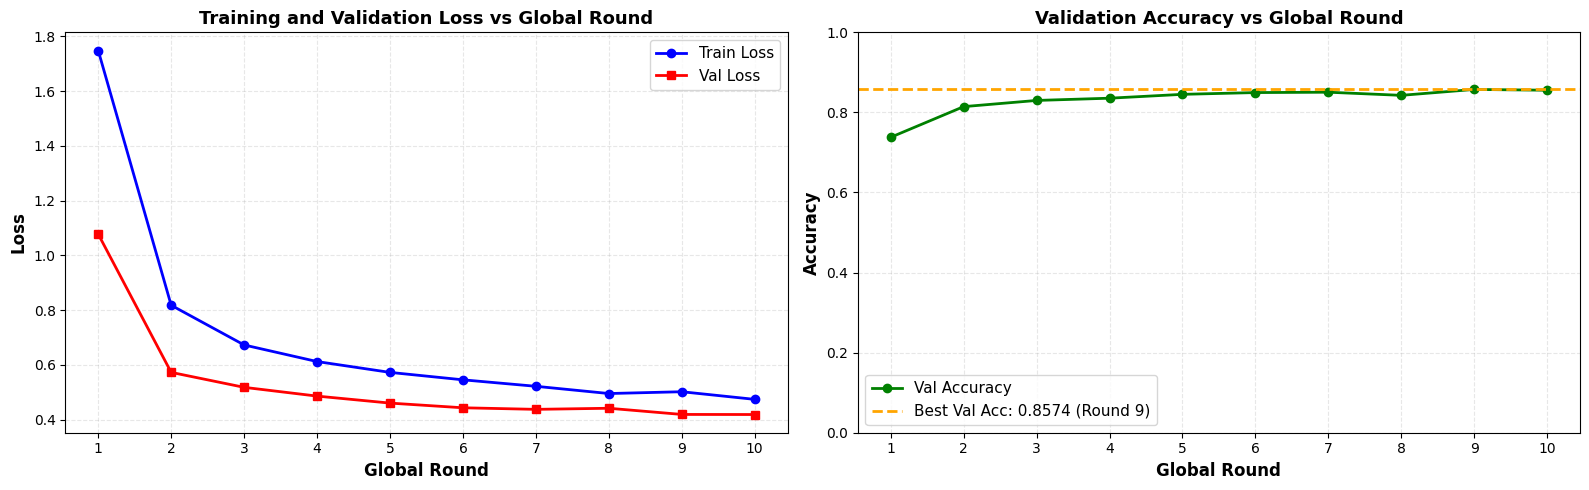
\includegraphics[width=\linewidth]{retrained_cifar_plots.png}
    \caption{
        \textbf{SGD with Momentum on CIFAR-10 (Retrained with Best Hyperparameters).} 
        Train Loss: $\mathbf{0.4742}$,\;
        Val Loss: $\mathbf{0.4188}$,\;
        Val Acc: $\mathbf{0.8554}$.
    }
    \label{fig:sgd_momentum_retrained}
\end{figure}

    \section{Experimental Results and Visualizations}
    \label{sec:appendix_plots}

    This section presents experimental visualizations for each optimizer variant evaluated on FEMNIST. Each figure contains multiple subfigures showing different aspects of the training process:
    \begin{itemize}
        \item \textbf{TVL (Training/Validation Loss):} Shows training loss, validation loss, and validation accuracy curves over communication rounds.
        \item \textbf{HYPER (Hyperparameter Importance):} Displays the relative importance of hyperparameters as determined by Optuna's analysis.
        \item \textbf{TOP (Top 5 Trials):} Compares the performance of the top 5 hyperparameter configurations.
    \end{itemize}

    \begin{figure}[h!]
        \centering
        \begin{subfigure}[b]{0.32\textwidth}
            \includegraphics[width=\textwidth]{PLOTS/SGD TVL.png}
            \caption{Training/Validation curves}
        \end{subfigure}
        \hfill
        \begin{subfigure}[b]{0.32\textwidth}
            \includegraphics[width=\textwidth]{PLOTS/SGD HYPER.png}
            \caption{Hyperparameter importance}
        \end{subfigure}
        \hfill
        \begin{subfigure}[b]{0.32\textwidth}
            \includegraphics[width=\textwidth]{PLOTS/SGD TOP.png}
            \caption{Top 5 trials comparison}
        \end{subfigure}
        \caption{SGD experimental results on FEMNIST.}
        \label{fig:sgd_plots}
    \end{figure}

    \begin{figure}[h!]
        \centering
        \begin{subfigure}[b]{0.32\textwidth}
            \includegraphics[width=\textwidth]{PLOTS/SGD MOMENTUM TVL.png}
            \caption{Training/Validation curves}
        \end{subfigure}
        \hfill
        \begin{subfigure}[b]{0.32\textwidth}
            \includegraphics[width=\textwidth]{PLOTS/SGD MOMENTUM HYPER.png}
            \caption{Hyperparameter importance}
        \end{subfigure}
        \hfill
        \begin{subfigure}[b]{0.32\textwidth}
            \includegraphics[width=\textwidth]{PLOTS/SGD MOMENTUM TOP.png}
            \caption{Top 5 trials comparison}
        \end{subfigure}
        \caption{SGD with Momentum experimental results on FEMNIST.}
        \label{fig:sgd_momentum_plots}
    \end{figure}

    \begin{figure}[h!]
        \centering
        \begin{subfigure}[b]{0.45\textwidth}
            \includegraphics[width=\textwidth]{PLOTS/ADAGRAD HYPER.png}
            \caption{Hyperparameter importance}
        \end{subfigure}
        \hfill
        \begin{subfigure}[b]{0.45\textwidth}
            \includegraphics[width=\textwidth]{PLOTS/ADAGRAD TOP.png}
            \caption{Top 5 trials comparison}
        \end{subfigure}
        \caption{Adagrad experimental results on FEMNIST.}
        \label{fig:adagrad_plots}
    \end{figure}

    \begin{figure}[h!]
        \centering
        \begin{subfigure}[b]{0.45\textwidth}
            \includegraphics[width=\textwidth]{PLOTS/ADAM TVL.png}
            \caption{Training/Validation curves}
        \end{subfigure}
        \hfill
        \begin{subfigure}[b]{0.45\textwidth}
            \includegraphics[width=\textwidth]{PLOTS/ADAM HYPER.png}
            \caption{Hyperparameter importance}
        \end{subfigure}
        \caption{Adam experimental results on FEMNIST.}
        \label{fig:adam_plots}
    \end{figure}

    \begin{figure}[h!]
        \centering
        \begin{subfigure}[b]{0.32\textwidth}
            \includegraphics[width=\textwidth]{PLOTS/ADAMW TVL.png}
            \caption{Training/Validation curves}
        \end{subfigure}
        \hfill
        \begin{subfigure}[b]{0.32\textwidth}
            \includegraphics[width=\textwidth]{PLOTS/ADAMW HYPER.png}
            \caption{Hyperparameter importance}
        \end{subfigure}
        \hfill
        \begin{subfigure}[b]{0.32\textwidth}
            \includegraphics[width=\textwidth]{PLOTS/ADAMW TOP.png}
            \caption{Top 5 trials comparison}
        \end{subfigure}
        \caption{AdamW experimental results on FEMNIST.}
        \label{fig:adamw_plots}
    \end{figure}

    \begin{figure}[h!]
        \centering
        \begin{subfigure}[b]{0.32\textwidth}
            \includegraphics[width=\textwidth]{PLOTS/RADAM TVL.png}
            \caption{Training/Validation curves}
        \end{subfigure}
        \hfill
        \begin{subfigure}[b]{0.32\textwidth}
            \includegraphics[width=\textwidth]{PLOTS/RADAM HYPER.png}
            \caption{Hyperparameter importance}
        \end{subfigure}
        \hfill
        \begin{subfigure}[b]{0.32\textwidth}
            \includegraphics[width=\textwidth]{PLOTS/RADAM TOP.png}
            \caption{Top 5 trials comparison}
        \end{subfigure}
        \caption{RAdam experimental results on FEMNIST.}
        \label{fig:radam_plots}
    \end{figure}

    \begin{figure}[h!]
        \centering
        \begin{subfigure}[b]{0.32\textwidth}
            \includegraphics[width=\textwidth]{PLOTS/RMSPROP TVL.png}
            \caption{Training/Validation curves}
        \end{subfigure}
        \hfill
        \begin{subfigure}[b]{0.32\textwidth}
            \includegraphics[width=\textwidth]{PLOTS/RMSPROP HYPER.png}
            \caption{Hyperparameter importance}
        \end{subfigure}
        \hfill
        \begin{subfigure}[b]{0.32\textwidth}
            \includegraphics[width=\textwidth]{PLOTS/RMSPROP TOP.png}
            \caption{Top 5 trials comparison}
        \end{subfigure}
        \caption{RMSProp experimental results on FEMNIST.}
        \label{fig:rmsprop_plots}
    \end{figure}

    {\small
    \begin{thebibliography}{9}

    \bibitem{mcmahan2017fedavg}
    H.~B. McMahan, E.~Moore, D.~Ramage, S.~Hampson, and B.~A. y Arcas.
    \newblock Communication-efficient learning of deep networks from decentralized data.
    \newblock In \emph{AISTATS}, 2017.

    \bibitem{li2020fedprox}
    T.~Li, A.~S. Sahu, M.~Zaheer, M.~Sanjabi, A.~Talwalkar, and V.~Smith.
    \newblock Federated optimization in heterogeneous networks.
    \newblock In \emph{MLSys}, 2020.

    \bibitem{kingma2014adam}
    D.~P. Kingma and J.~Ba.
    \newblock Adam: A method for stochastic optimization.
    \newblock In \emph{ICLR}, 2015.

    \bibitem{wu2018groupnorm}
    Y.~Wu and K.~He.
    \newblock Group normalization.
    \newblock In \emph{ECCV}, 2018.

    \bibitem{hsieh2020quagmire}
    K.~Hsieh, A.~Phanishayee, O.~Mutlu, and P.~B. Gibbons.
    \newblock The non-{IID} data quagmire of decentralized machine learning.
    \newblock In \emph{ICML}, 2020.

    \end{thebibliography}
    }

    \end{document}
